\section{Programos sudarymas ir rezultatai}

Pagal dviejų dimensijų skaitinį modelį \eqref{numerical-eqs} sudarytas uždavinį sprendžiantis skriptas ir kiti pagalbiniai skriptai duomenims vaizduoti ir tikrinti. Skriptai rašomi \textit{Python} programavimo kalba, naudojant \textit{NumPy}, \textit{SciPy}, \textit{Matplotlib} paketus. 

Modelio rezultatai yra saugomi kaip atskiri \textit{.npy} formato failai, kurie yra skirti saugoti \mbox{\textit{NumPy}} masyvus. Dėl praktinių rezultatų panaudojimo ir tyrimo nebūtina saugoti informacijos apie visus laiko žingsnius, todėl išsaugotuose rezultatų failuose, simuliacijos kadrai laiko kryptimi gali būti praretinti iki tūkstančio kartų, priklausomai nuo pasirinktų parametrų. Pagalbiniai duomenų vaizdavimo skriptai šiuos duomenis agreguoja į grafikus, kurie išsaugomi \textit{.png} formatu.

\begin{figure}[h!]
\centering
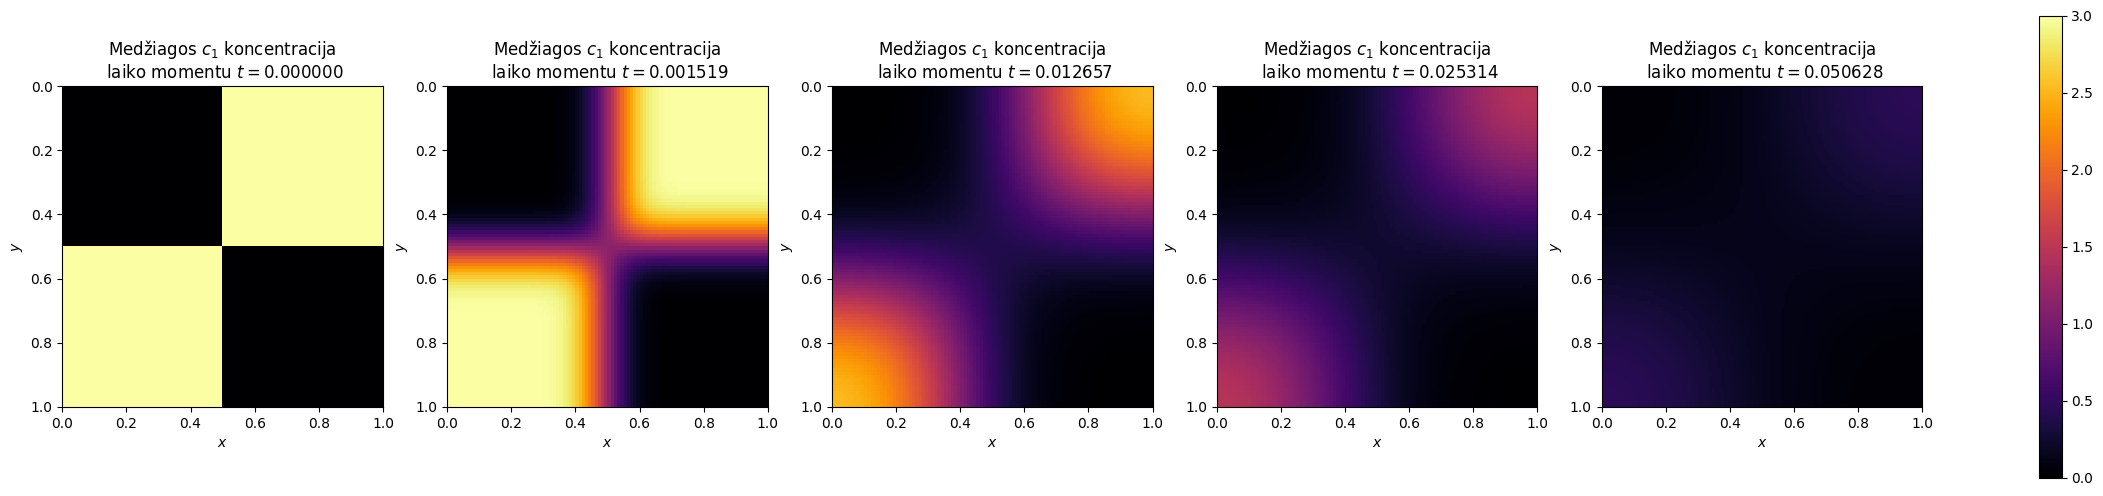
\includegraphics[width=\textwidth]{../assets/examples-c1.png} \\
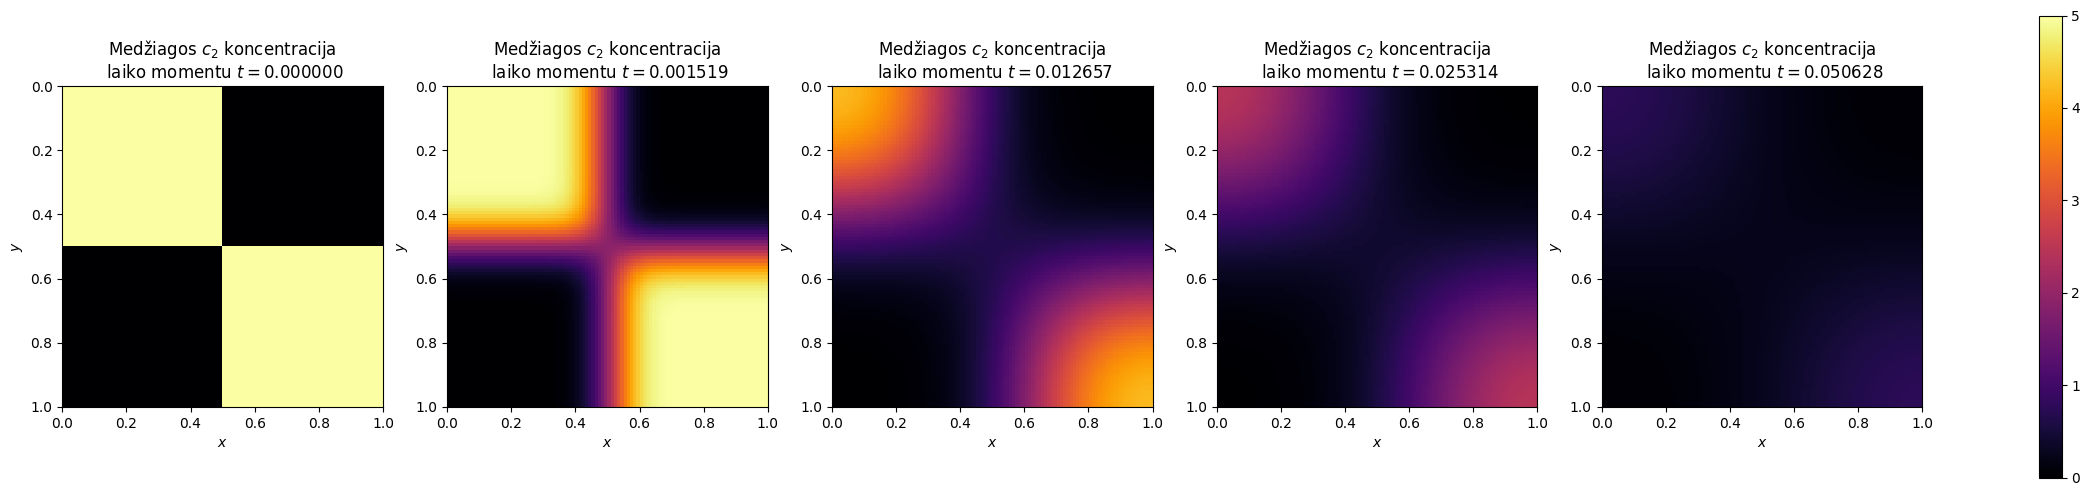
\includegraphics[width=\textwidth]{../assets/examples-c2.png} \\
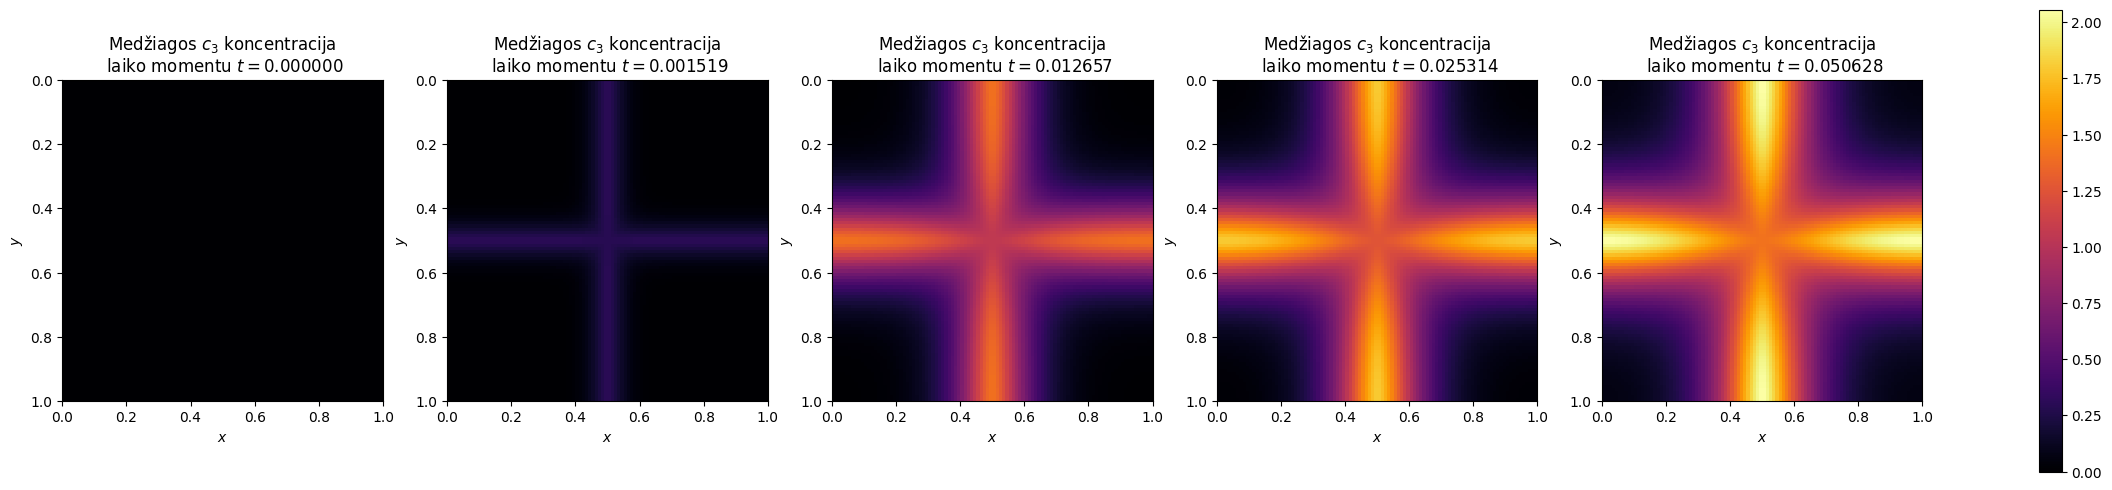
\includegraphics[width=\textwidth]{../assets/examples-c3.png}
\caption{Kompiuterinio modelio rezultato pavyzdys. $D = 0.05$, $W = 1$, $H = 1$, $\Delta x = \frac{1}{99}$, $\Delta y = \frac{1}{99}$, $k = 1$, $c_0 = 1$.}
%     \label{result-example}
\end{figure}

\subsection{Rezultatų korektiškumo tikrinimas}
\subsection{Palyginimas su eksperimentiniais duomenimis}
